\documentclass[]{report}

\usepackage{graphicx}
\usepackage{float}
\usepackage{amsmath}
\usepackage{amsfonts}
\usepackage{wasysym}
\usepackage{listings}
\usepackage{xcolor}
\lstset{
	basicstyle=\ttfamily,
	columns=fullflexible,
	frame=L,
	showstringspaces=false, 
	commentstyle=\color{green},
	breaklines=true,
	postbreak=\mbox{\textcolor{red}{$\hookrightarrow$}\space},
}
\pagenumbering{Roman}
% Title Page
\title{MCEN 3047 - Homework 3}
\author{Jack Reilly Goldrick}


\begin{document}
	\maketitle
	
	
	\section{Problem 1}
	
	
		\begin{figure}[H]
			\centering
			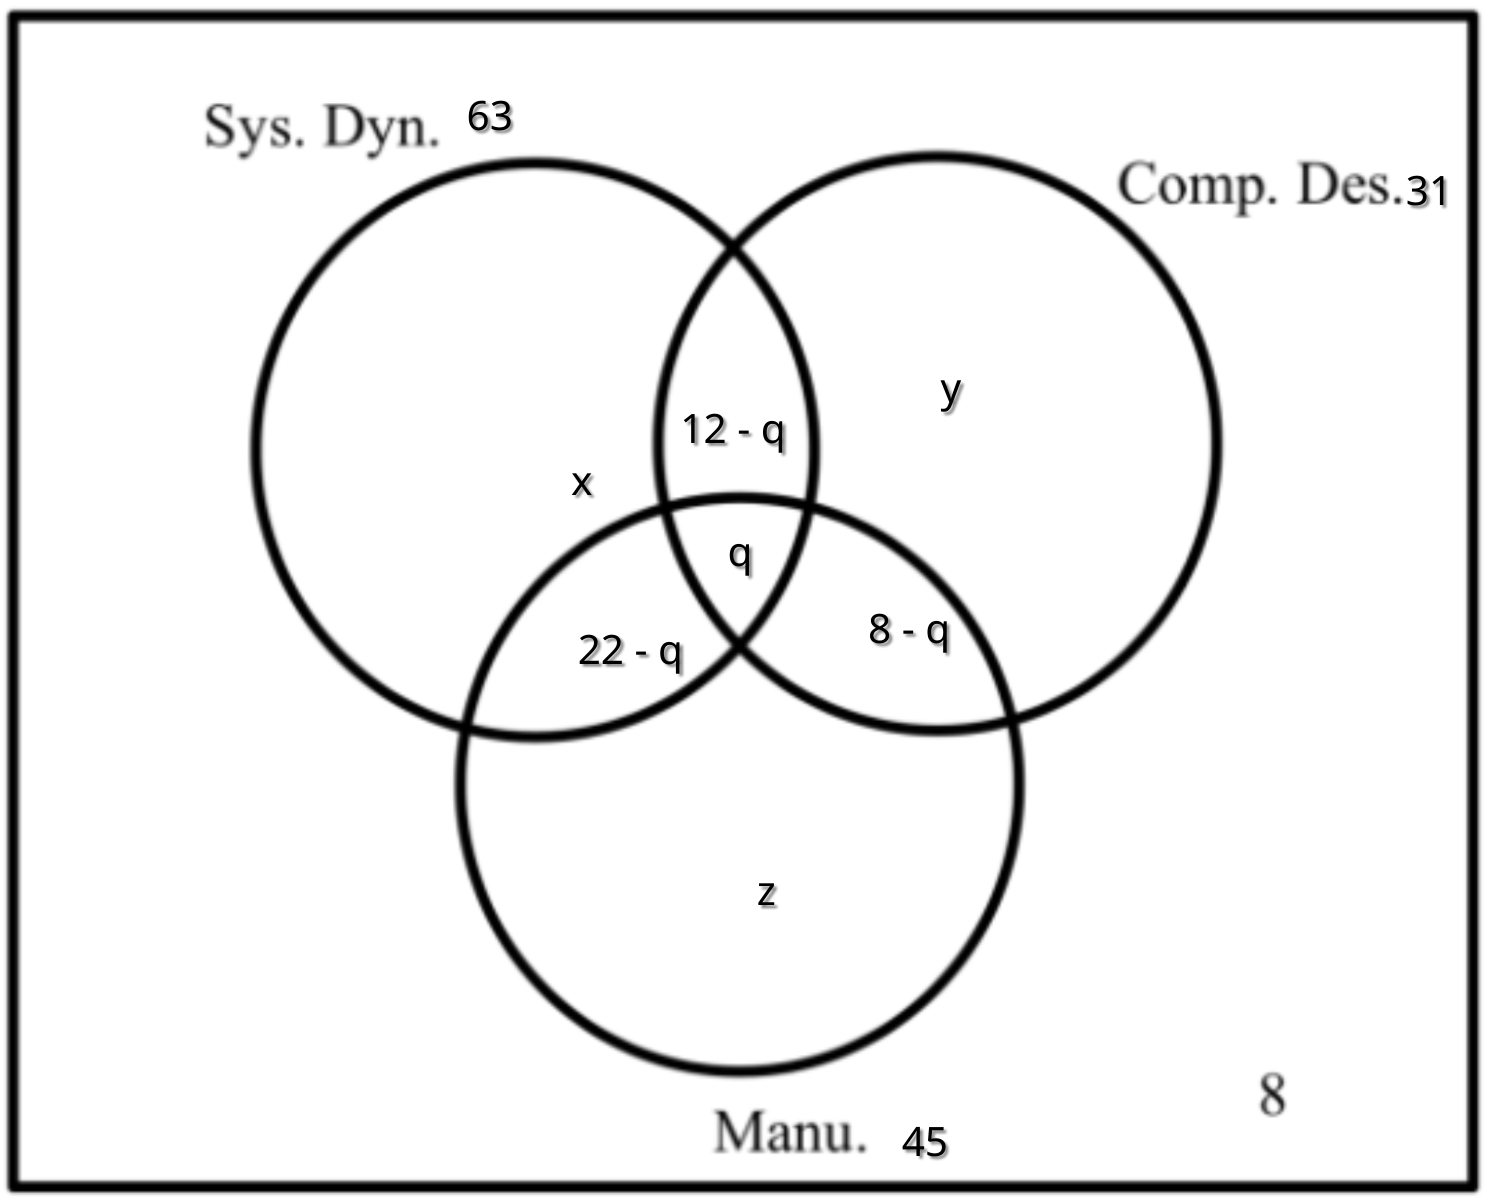
\includegraphics[width=0.7\linewidth]{./pics/1}
		\end{figure}
	
		\subsection{Part A}
			\begin{itemize}
				\item Solving the following system of equations yields the following result:
				$$ |SysD \cap Manu \cap CompD | = 3 $$
			\end{itemize}
			
			
			\subsection{Part B}
			
			
					\begin{figure}[H]
						\centering
							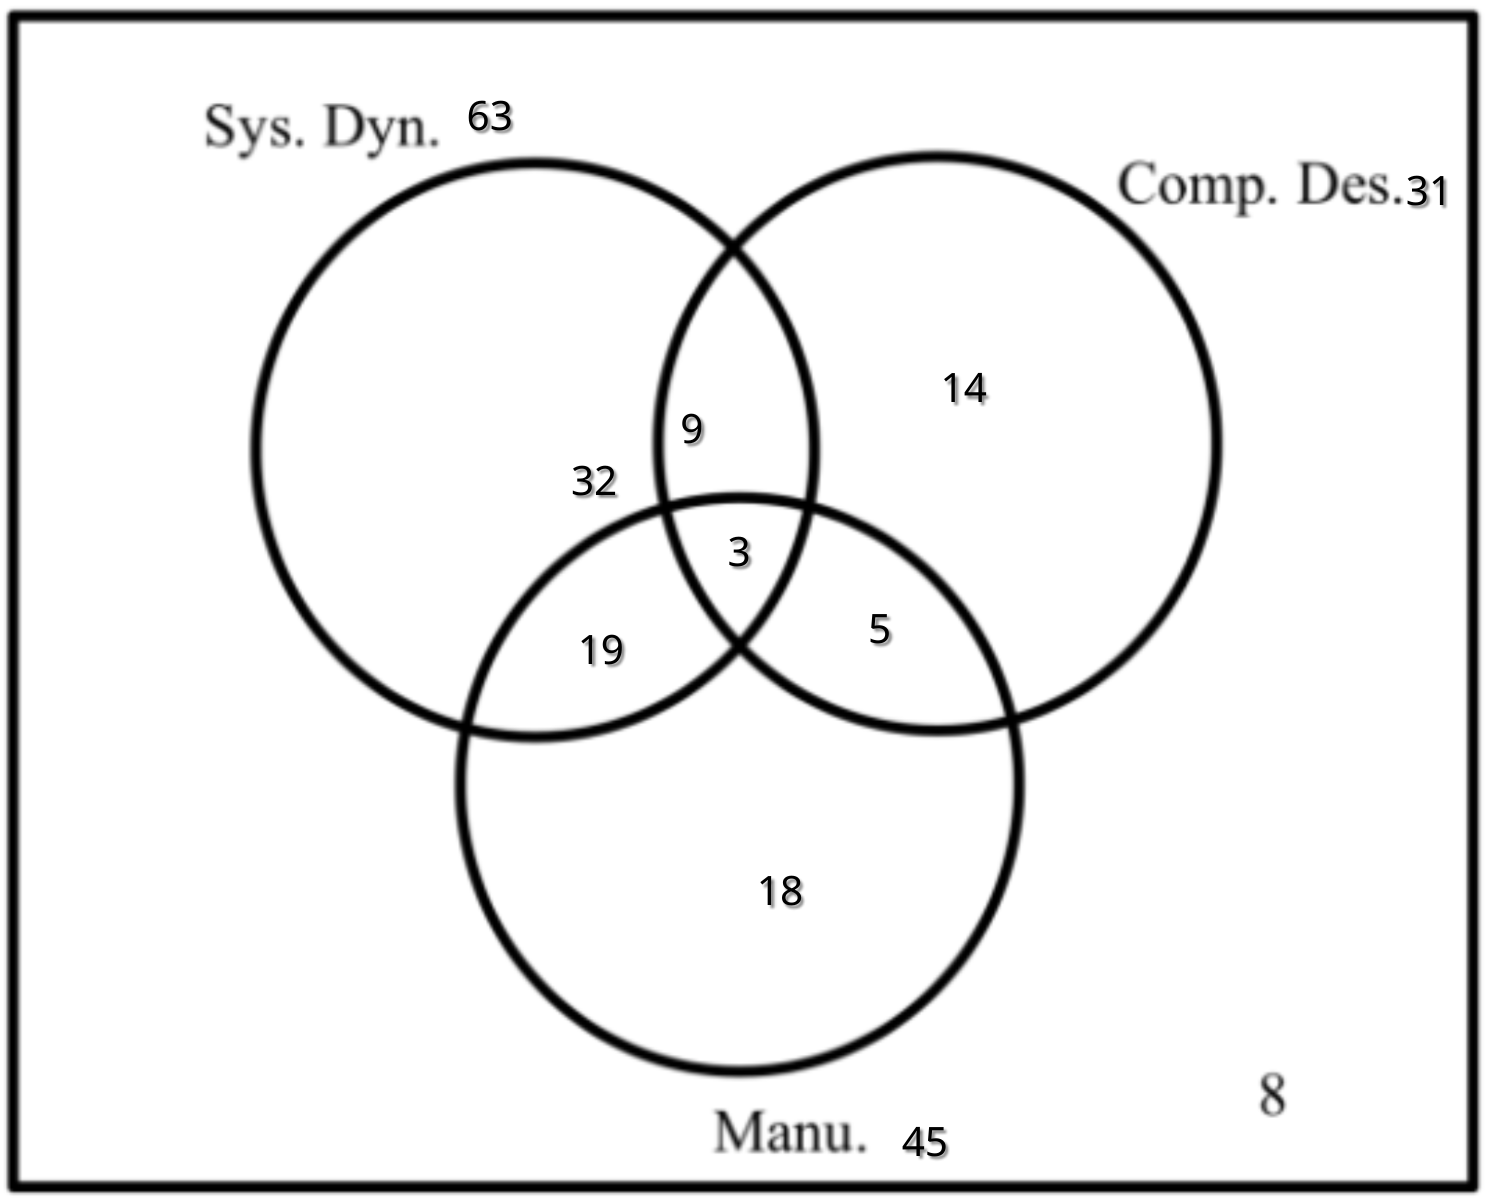
\includegraphics[width=0.7\linewidth]{./pics/1.b}
					\end{figure}


			\subsection{Part C}
			
			$$ P = \frac{32}{108}$$
			
			$$ P =  29.6 \% $$
			
			
			\subsection{Part D}
			
			
			$$ P = \frac{9}{108} $$
			
			$$P = 8.3\%$$
			
			\subsection{Part E}
			
			
			$$ P = \frac{\frac{22}{108}}{\frac{45}{108}} $$
			
			$$ P = 48.889 \% $$
			
			\subsection{Part F}
			
			$$ P = \frac{\frac{22}{108}}{\frac{63}{108}} $$
			
			$$ P = 34.92\% $$
			
			
			\newpage
			
			
		\section{Problem 2}
		
		\subsection{Part A}
		
		$$ \frac{\partial \delta}{\partial I} = - \frac{P L^3}{3 E I^2} $$
		
		$$ \frac{\partial \delta}{\partial L} = \frac{P L^2}{ E I} $$
		
		
		$$ \sigma_{\delta} = \sqrt{   (\frac{P L^3}{3 E I^2})^2  (\sigma_{I})^2   + (\frac{P L^2}{ E I})^2   (\sigma_{L})^2}$$
		
		$$ \sigma_{\delta} = . 67998 \text{cm} $$
		
		
		\subsection{Part B}
		
		The code returns the deflection of the beam as 2.94e-02 m with an error of 6.72046e-03 m.
		
		
		\newpage
		
		
		
	\section{Problem 3}
	
	
	
	The spring constant is 10.04 N/m with an uncertainty of 0.2064 N/m.
	\newline
	The Damping constant is 3.06 N/m/s with an uncertainty of 0.0561 N/m/s.
	
	
	\newpage
	
	\section{Problem 4}
	
	\begin{itemize}
		\item Question: What happens to the least squares solution $x$ of $b = Ax$ when A is an orthogonal matrix (A matrix with Orthonormal Basis Vectors):
		
				\subitem[1.] $x = A^T b$
				
				\subitem[2.] $x = (A^T A)^{-1}  A^T b$
				
				\subitem[3.] $x = (A^T A)^{-1} b$
				
				\subitem[4.] $x = (A^T A) b$
				
				
			\item Answer [1.]
	\end{itemize}
	
	\newpage
	
	\section{Code}
	
	
	\lstinputlisting[language=python]{../src/set_3.py}
	
	
	
\end{document}          
